% network: four labeled nodes on a closed ring; single elliptical loop, no arrows, no weights.
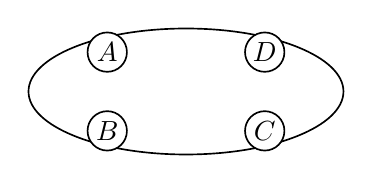
\begin{tikzpicture}[line width=.6pt,font=\normalsize]
\tikzset{nd/.style={circle,draw,fill=white,minimum size=5mm,inner sep=0pt}}
\draw (0,0) ellipse (20mm and 8mm);
\node[nd] (A) at (-10mm,5mm) {$A$};
\node[nd] (D) at (10mm,5mm) {$D$};
\node[nd] (B) at (-10mm,-5mm) {$B$};
\node[nd] (C) at (10mm,-5mm) {$C$};
\end{tikzpicture}
